\section{Linear TM Overlay}

\subsection{Architecture Description}
A linear array of FUs as a time-multiplexed (TM) overlay has been proposed~\cite{li2018time} where each FU can be time multiplexed among operations present in a single scheduling stage of a directed acyclic graph (DAG). 
The 32-bit linear TM overlay is comprised of a quasi-streaming data interface made up of two FIFO channels implemented using Block RAMs, which transmit the data through daisy-chained fully pipelined time-multiplexed FUs, as shown in Figure~\ref{overlay}. 
By eliminating the fully flexible routability of the CGRA-like overlays, the linear TM overlay can achieve a very area efficient design, representing less than 6\% of the logic and DSP resources on Zynq. 
The initiation interval (II) can be significantly reduced by making some minor architectural enhancements, such as adding a rotating register file and replicating the data stream. 
These changes result in a peak throughput of 1.8 GOPS. 
Adding write-back capabilities to the FU design reduces the overlay depth requirement by allowing multiple nodes on the critical path to be combined. 
This also eliminates the need to reconfigure the overlay whenever the application kernel changes, making the overlay suitable for more general purpose applications. 


\begin{figure}
    \centering
	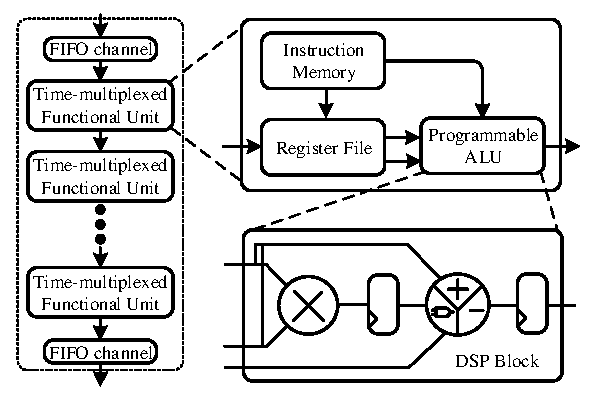
\includegraphics[width=\columnwidth]{Figures/overlay.pdf}
	\caption{A linear TM overlay.}
	\label{overlay}
\end{figure}


\subsection{Overlay Control}
A back-pressure control circuit is built around the input FIFO channel to manage the functionality of the linear TM overlay, as shown in Figure~\ref{back_pressure}. 
There are three control signals which indicate the duration for instruction load, overlay setup and data write respectively, referred to as \textit{inst\_load}, \textit{reg\_wren}, and \textit{data\_wren}. 
Initially, FU instructions are read from the memory and streamed through the daisy-chained FUs. 
During instruction load (when the \textit{inst\_load} is high), both the write enable port of the FIFO and the valid signal (\textit{valid\_out}) for data output are disabled. 
After instruction load, two integers are written to the back-pressure control circuit. 
The first represents the number of data words to be input to the first FU for a specific compute kernel while the other is equal to the II minus one (II-1) and determines the interval between data loads. 
These values are written into the controller when the \textit{reg\_wren} signal is active.
%The process of instruction load and overlay setup represent the initialization of the overlay.

The dashed box on the LHS of Figure~\ref{back_pressure} acts as the control module for the write enable port of the FIFO, while the other dashed box on the RHS contains the logic to control the read enable port of the FIFO. 
Data is written into the FIFO when \textit{wr\_en} is high.
The read enable signal (\textit{rd\_en}) for the FIFO is generated from a counter which determines the number of cycles needed to load input data to the FU. 
The counter starts counting from 0 when the \textit{empty} signal goes low (indicating that data is available in the FIFO). The counter counts up until the count value equals II-1, at which point it rolls over back to zero.   
The \textit{rd\_en} signal is valid only while the counter is less than the initial number loaded into the back-pressure circuit, limiting the amount of data to be loaded into the first FU.
Once the counter value is greater than or equal to the data load number (in the back-pressure circuit), the \textit{rd\_en} signal is forced low and the input data is buffered in the FIFO.


\begin{figure}
	\centering
	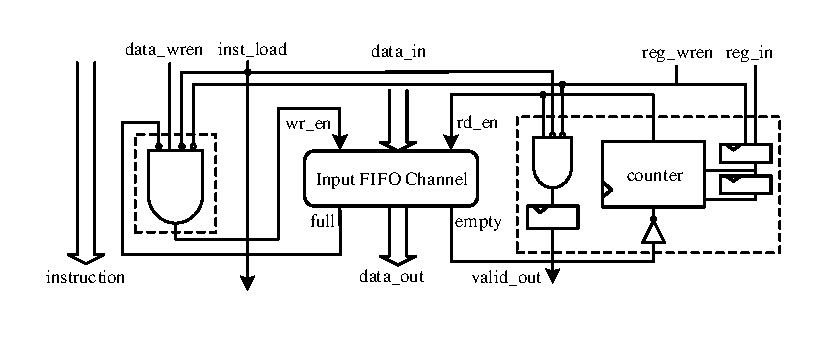
\includegraphics[width=\columnwidth]{Figures/control.pdf}
	\caption{Back-pressure control circuit.}
	\label{back_pressure}
\end{figure}
	

\subsection{What is Needed for a Full Working Implementation?}
The linear TM overlay has shown its advantages to implement an area efficient design with fast context switch and comparable high throughput. 
However, to demonstrate the suitability of the overlay as an FPGA accelerator, it is important to develop a memory interface between the processor/memory subsystems and the overlay which is able to provide high-bandwidth data transmission. 
As discussed in the previous section, two stream interfaces are required for transmitting the data between the host processor and the overlay accelerator. 
Additionally, it is necessary to set up memory arrays or registers so that the user has access to control the overlay system, i.e. the instruction load, overlay setup, and data write. 

